\documentclass{extbook}[14pt]
\usepackage{multicol, enumerate, enumitem, hyperref, color, soul, setspace, parskip, fancyhdr, amssymb, amsthm, amsmath, latexsym, units, mathtools}
\everymath{\displaystyle}
\usepackage[headsep=0.5cm,headheight=0cm, left=1 in,right= 1 in,top= 1 in,bottom= 1 in]{geometry}
\usepackage{dashrule}  % Package to use the command below to create lines between items
\newcommand{\litem}[1]{\item #1

\rule{\textwidth}{0.4pt}}
\pagestyle{fancy}
\lhead{}
\chead{Answer Key for Makeup Progress Quiz 2 Version C}
\rhead{}
\lfoot{2790-1423}
\cfoot{}
\rfoot{Summer C 2021}
\begin{document}
\textbf{This key should allow you to understand why you choose the option you did (beyond just getting a question right or wrong). \href{https://xronos.clas.ufl.edu/mac1105spring2020/courseDescriptionAndMisc/Exams/LearningFromResults}{More instructions on how to use this key can be found here}.}

\textbf{If you have a suggestion to make the keys better, \href{https://forms.gle/CZkbZmPbC9XALEE88}{please fill out the short survey here}.}

\textit{Note: This key is auto-generated and may contain issues and/or errors. The keys are reviewed after each exam to ensure grading is done accurately. If there are issues (like duplicate options), they are noted in the offline gradebook. The keys are a work-in-progress to give students as many resources to improve as possible.}

\rule{\textwidth}{0.4pt}

\begin{enumerate}\litem{
Which of the following equations \textit{could} be of the graph presented below?

\begin{center}
    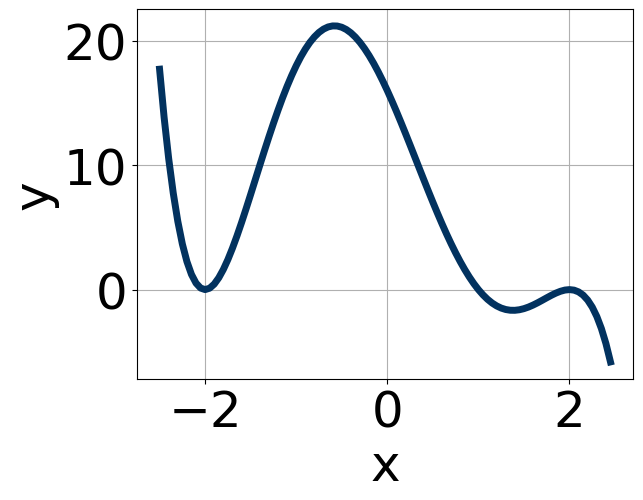
\includegraphics[width=0.5\textwidth]{../Figures/polyGraphToFunctionC.png}
\end{center}


The solution is \( -6(x - 2)^{10} (x + 2)^{4} (x - 1)^{7} \), which is option D.\begin{enumerate}[label=\Alph*.]
\item \( -13(x - 2)^{10} (x + 2)^{5} (x - 1)^{10} \)

The factor $(x + 2)$ should have an even power and the factor $(x - 1)$ should have an odd power.
\item \( -14(x - 2)^{10} (x + 2)^{9} (x - 1)^{11} \)

The factor $(x + 2)$ should have an even power.
\item \( 18(x - 2)^{10} (x + 2)^{4} (x - 1)^{10} \)

The factor $(x - 1)$ should have an odd power and the leading coefficient should be the opposite sign.
\item \( -6(x - 2)^{10} (x + 2)^{4} (x - 1)^{7} \)

* This is the correct option.
\item \( 16(x - 2)^{8} (x + 2)^{8} (x - 1)^{5} \)

This corresponds to the leading coefficient being the opposite value than it should be.
\end{enumerate}

\textbf{General Comment:} General Comments: Draw the x-axis to determine which zeros are touching (and so have even multiplicity) or cross (and have odd multiplicity).
}
\litem{
Construct the lowest-degree polynomial given the zeros below. Then, choose the intervals that contain the coefficients of the polynomial in the form $ax^3+bx^2+cx+d$.
\[ \frac{-3}{5}, \frac{7}{4}, \text{ and } \frac{1}{3} \]The solution is \( 60x^{3} -89 x^{2} -40 x + 21 \), which is option B.\begin{enumerate}[label=\Alph*.]
\item \( a \in [53, 63], b \in [-91, -78], c \in [-46, -37], \text{ and } d \in [-21, -18] \)

$60x^{3} -89 x^{2} -40 x -21$, which corresponds to multiplying everything correctly except the constant term.
\item \( a \in [53, 63], b \in [-91, -78], c \in [-46, -37], \text{ and } d \in [20, 23] \)

* $60x^{3} -89 x^{2} -40 x + 21$, which is the correct option.
\item \( a \in [53, 63], b \in [83, 95], c \in [-46, -37], \text{ and } d \in [-21, -18] \)

$60x^{3} +89 x^{2} -40 x -21$, which corresponds to multiplying out $(5x -3)(4x + 7)(3x + 1)$.
\item \( a \in [53, 63], b \in [49, 51], c \in [-88, -79], \text{ and } d \in [20, 23] \)

$60x^{3} +49 x^{2} -86 x + 21$, which corresponds to multiplying out $(5x -3)(4x + 7)(3x -1)$.
\item \( a \in [53, 63], b \in [-165, -159], c \in [107, 112], \text{ and } d \in [-21, -18] \)

$60x^{3} -161 x^{2} +110 x -21$, which corresponds to multiplying out $(5x -3)(4x -7)(3x -1)$.
\end{enumerate}

\textbf{General Comment:} To construct the lowest-degree polynomial, you want to multiply out $(5x + 3)(4x -7)(3x -1)$
}
\litem{
Describe the zero behavior of the zero $x = 8$ of the polynomial below.
\[ f(x) = 3(x + 8)^{8}(x - 8)^{11}(x - 7)^{9}(x + 7)^{13} \]The solution is the graph below, which is option D.
    \begin{center}
        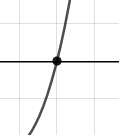
\includegraphics[width=0.3\textwidth]{../Figures/polyZeroBehaviorCopyDC.png}
    \end{center}\begin{enumerate}[label=\Alph*.]
\begin{multicols}{2}
\item 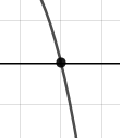
\includegraphics[width = 0.3\textwidth]{../Figures/polyZeroBehaviorCopyAC.png}
\item 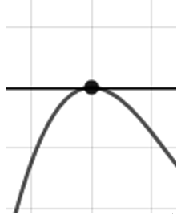
\includegraphics[width = 0.3\textwidth]{../Figures/polyZeroBehaviorCopyBC.png}
\item 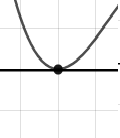
\includegraphics[width = 0.3\textwidth]{../Figures/polyZeroBehaviorCopyCC.png}
\item 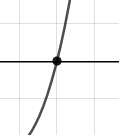
\includegraphics[width = 0.3\textwidth]{../Figures/polyZeroBehaviorCopyDC.png}
\end{multicols}\item None of the above.\end{enumerate}
\textbf{General Comment:} You will need to sketch the entire graph, then zoom in on the zero the question asks about.
}
\litem{
Describe the end behavior of the polynomial below.
\[ f(x) = -4(x + 6)^{4}(x - 6)^{5}(x + 2)^{5}(x - 2)^{5} \]The solution is the graph below, which is option A.
    \begin{center}
        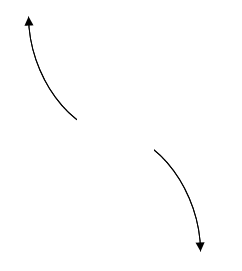
\includegraphics[width=0.3\textwidth]{../Figures/polyEndBehaviorCopyAC.png}
    \end{center}\begin{enumerate}[label=\Alph*.]
\begin{multicols}{2}
\item 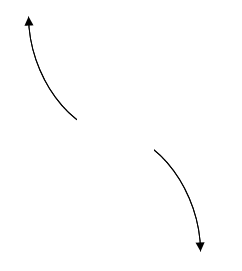
\includegraphics[width = 0.3\textwidth]{../Figures/polyEndBehaviorCopyAC.png}
\item 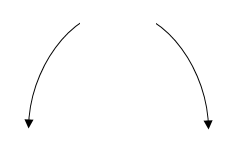
\includegraphics[width = 0.3\textwidth]{../Figures/polyEndBehaviorCopyBC.png}
\item 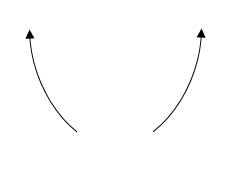
\includegraphics[width = 0.3\textwidth]{../Figures/polyEndBehaviorCopyCC.png}
\item 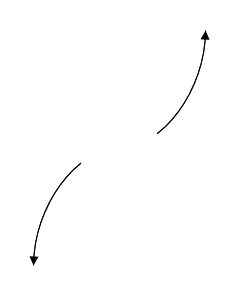
\includegraphics[width = 0.3\textwidth]{../Figures/polyEndBehaviorCopyDC.png}
\end{multicols}\item None of the above.\end{enumerate}
\textbf{General Comment:} Remember that end behavior is determined by the leading coefficient AND whether the \textbf{sum} of the multiplicities is positive or negative.
}
\litem{
Describe the end behavior of the polynomial below.
\[ f(x) = 4(x + 2)^{5}(x - 2)^{8}(x + 9)^{3}(x - 9)^{3} \]The solution is the graph below, which is option D.
    \begin{center}
        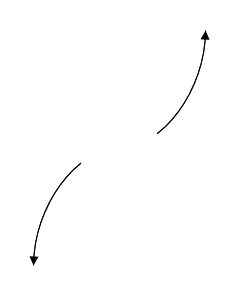
\includegraphics[width=0.3\textwidth]{../Figures/polyEndBehaviorDC.png}
    \end{center}\begin{enumerate}[label=\Alph*.]
\begin{multicols}{2}
\item 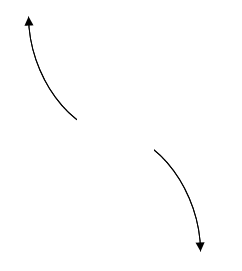
\includegraphics[width = 0.3\textwidth]{../Figures/polyEndBehaviorAC.png}
\item 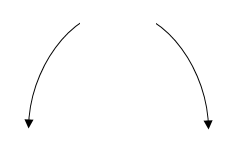
\includegraphics[width = 0.3\textwidth]{../Figures/polyEndBehaviorBC.png}
\item 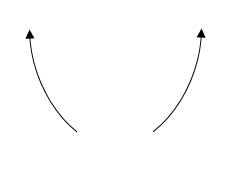
\includegraphics[width = 0.3\textwidth]{../Figures/polyEndBehaviorCC.png}
\item 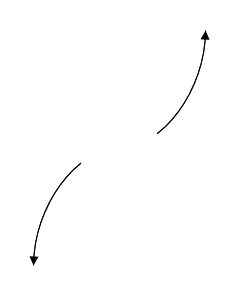
\includegraphics[width = 0.3\textwidth]{../Figures/polyEndBehaviorDC.png}
\end{multicols}\item None of the above.\end{enumerate}
\textbf{General Comment:} Remember that end behavior is determined by the leading coefficient AND whether the \textbf{sum} of the multiplicities is positive or negative.
}
\litem{
Construct the lowest-degree polynomial given the zeros below. Then, choose the intervals that contain the coefficients of the polynomial in the form $x^3+bx^2+cx+d$.
\[ -5 + 5 i \text{ and } -1 \]The solution is \( x^{3} +11 x^{2} +60 x + 50 \), which is option B.\begin{enumerate}[label=\Alph*.]
\item \( b \in [-16, -10], c \in [59, 67], \text{ and } d \in [-58, -48] \)

$x^{3} -11 x^{2} +60 x -50$, which corresponds to multiplying out $(x-(-5 + 5 i))(x-(-5 - 5 i))(x -1)$.
\item \( b \in [4, 19], c \in [59, 67], \text{ and } d \in [46, 58] \)

* $x^{3} +11 x^{2} +60 x + 50$, which is the correct option.
\item \( b \in [-8, 6], c \in [-1, 13], \text{ and } d \in [3, 6] \)

$x^{3} + x^{2} +6 x + 5$, which corresponds to multiplying out $(x + 5)(x + 1)$.
\item \( b \in [-8, 6], c \in [-6, 3], \text{ and } d \in [-7, 3] \)

$x^{3} + x^{2} -4 x -5$, which corresponds to multiplying out $(x -5)(x + 1)$.
\item \( \text{None of the above.} \)

This corresponds to making an unanticipated error or not understanding how to use nonreal complex numbers to create the lowest-degree polynomial. If you chose this and are not sure what you did wrong, please contact the coordinator for help.
\end{enumerate}

\textbf{General Comment:} Remember that the conjugate of $a+bi$ is $a-bi$. Since these zeros always come in pairs, we need to multiply out $(x-(-5 + 5 i))(x-(-5 - 5 i))(x-(-1))$.
}
\litem{
Construct the lowest-degree polynomial given the zeros below. Then, choose the intervals that contain the coefficients of the polynomial in the form $ax^3+bx^2+cx+d$.
\[ \frac{-2}{5}, \frac{-3}{2}, \text{ and } \frac{1}{5} \]The solution is \( 50x^{3} +85 x^{2} +11 x -6 \), which is option C.\begin{enumerate}[label=\Alph*.]
\item \( a \in [48, 62], b \in [44, 50], c \in [-44, -38], \text{ and } d \in [1, 10] \)

$50x^{3} +45 x^{2} -41 x + 6$, which corresponds to multiplying out $(5x -2)(2x + 3)(5x -1)$.
\item \( a \in [48, 62], b \in [-106, -98], c \in [42, 50], \text{ and } d \in [-8, 2] \)

$50x^{3} -105 x^{2} +49 x -6$, which corresponds to multiplying out $(5x -2)(2x -3)(5x -1)$.
\item \( a \in [48, 62], b \in [79, 88], c \in [7, 18], \text{ and } d \in [-8, 2] \)

* $50x^{3} +85 x^{2} +11 x -6$, which is the correct option.
\item \( a \in [48, 62], b \in [79, 88], c \in [7, 18], \text{ and } d \in [1, 10] \)

$50x^{3} +85 x^{2} +11 x + 6$, which corresponds to multiplying everything correctly except the constant term.
\item \( a \in [48, 62], b \in [-85, -84], c \in [7, 18], \text{ and } d \in [1, 10] \)

$50x^{3} -85 x^{2} +11 x + 6$, which corresponds to multiplying out $(5x -2)(2x -3)(5x + 1)$.
\end{enumerate}

\textbf{General Comment:} To construct the lowest-degree polynomial, you want to multiply out $(5x + 2)(2x + 3)(5x -1)$
}
\litem{
Which of the following equations \textit{could} be of the graph presented below?

\begin{center}
    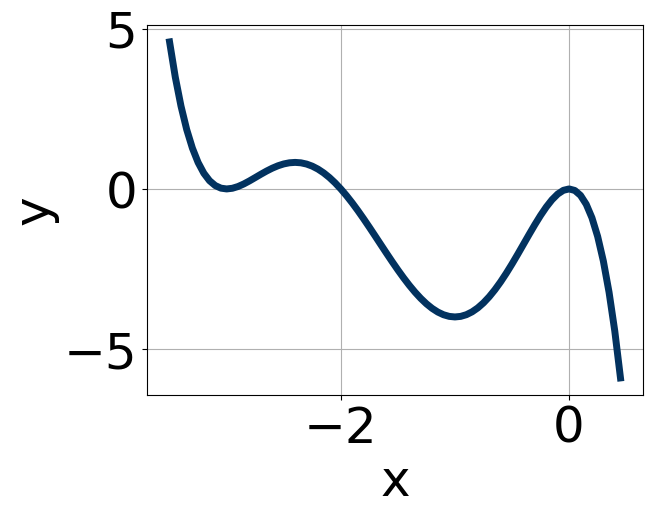
\includegraphics[width=0.5\textwidth]{../Figures/polyGraphToFunctionCopyC.png}
\end{center}


The solution is \( -13x^{8} (x + 3)^{10} (x + 2)^{5} \), which is option D.\begin{enumerate}[label=\Alph*.]
\item \( 14x^{10} (x + 3)^{10} (x + 2)^{5} \)

This corresponds to the leading coefficient being the opposite value than it should be.
\item \( 18x^{10} (x + 3)^{4} (x + 2)^{4} \)

The factor $(x + 2)$ should have an odd power and the leading coefficient should be the opposite sign.
\item \( -11x^{9} (x + 3)^{6} (x + 2)^{5} \)

The factor $x$ should have an even power.
\item \( -13x^{8} (x + 3)^{10} (x + 2)^{5} \)

* This is the correct option.
\item \( -8x^{11} (x + 3)^{10} (x + 2)^{10} \)

The factor $x$ should have an even power and the factor $(x + 2)$ should have an odd power.
\end{enumerate}

\textbf{General Comment:} General Comments: Draw the x-axis to determine which zeros are touching (and so have even multiplicity) or cross (and have odd multiplicity).
}
\litem{
Construct the lowest-degree polynomial given the zeros below. Then, choose the intervals that contain the coefficients of the polynomial in the form $x^3+bx^2+cx+d$.
\[ 4 - 3 i \text{ and } 3 \]The solution is \( x^{3} -11 x^{2} +49 x -75 \), which is option B.\begin{enumerate}[label=\Alph*.]
\item \( b \in [9, 12], c \in [40, 52], \text{ and } d \in [74, 86] \)

$x^{3} +11 x^{2} +49 x + 75$, which corresponds to multiplying out $(x-(4 - 3 i))(x-(4 + 3 i))(x + 3)$.
\item \( b \in [-14, -5], c \in [40, 52], \text{ and } d \in [-77, -72] \)

* $x^{3} -11 x^{2} +49 x -75$, which is the correct option.
\item \( b \in [0, 3], c \in [0, 5], \text{ and } d \in [-9, -8] \)

$x^{3} + x^{2} -9$, which corresponds to multiplying out $(x + 3)(x -3)$.
\item \( b \in [0, 3], c \in [-10, -6], \text{ and } d \in [7, 16] \)

$x^{3} + x^{2} -7 x + 12$, which corresponds to multiplying out $(x -4)(x -3)$.
\item \( \text{None of the above.} \)

This corresponds to making an unanticipated error or not understanding how to use nonreal complex numbers to create the lowest-degree polynomial. If you chose this and are not sure what you did wrong, please contact the coordinator for help.
\end{enumerate}

\textbf{General Comment:} Remember that the conjugate of $a+bi$ is $a-bi$. Since these zeros always come in pairs, we need to multiply out $(x-(4 - 3 i))(x-(4 + 3 i))(x-(3))$.
}
\litem{
Describe the zero behavior of the zero $x = 3$ of the polynomial below.
\[ f(x) = 3(x - 3)^{5}(x + 3)^{10}(x + 8)^{5}(x - 8)^{6} \]The solution is the graph below, which is option D.
    \begin{center}
        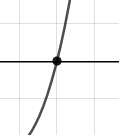
\includegraphics[width=0.3\textwidth]{../Figures/polyZeroBehaviorDC.png}
    \end{center}\begin{enumerate}[label=\Alph*.]
\begin{multicols}{2}
\item 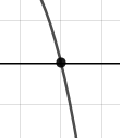
\includegraphics[width = 0.3\textwidth]{../Figures/polyZeroBehaviorAC.png}
\item 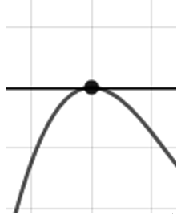
\includegraphics[width = 0.3\textwidth]{../Figures/polyZeroBehaviorBC.png}
\item 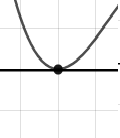
\includegraphics[width = 0.3\textwidth]{../Figures/polyZeroBehaviorCC.png}
\item 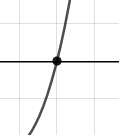
\includegraphics[width = 0.3\textwidth]{../Figures/polyZeroBehaviorDC.png}
\end{multicols}\item None of the above.\end{enumerate}
\textbf{General Comment:} You will need to sketch the entire graph, then zoom in on the zero the question asks about.
}
\end{enumerate}

\end{document}